\chapter{Contexte général et présentation du projet}

\section{Introduction}
Ce chapitre expose le cadre global dans lequel s'inscrit le projet. Il présente l'étude de l'existant, les critiques formulées et la solution proposée, ainsi que l'organisation adoptée pour sa réalisation. La planification opérationnelle est détaillée à l'aide d'outils formels tels que le tableau des tâches, la méthode PERT et le diagramme de Gantt, le tout structuré sous la méthodologie en Y du processus \textbf{2TUP} (2 Track Unified Process).

\section{Présentation du projet et étude de l'existant}
\subsection{Le recrutement digital au Maroc : Enjeux et Défis}
La digitalisation de l'économie marocaine a profondément modifié le secteur des ressources humaines. Auparavant cantonné aux annonces dans la presse écrite ou aux agences physiques, le recrutement s'est massivement déplacé vers le web. Les entreprises recherchent désormais une réduction des coûts de traitement, un sourcing plus rapide et une meilleure qualification des profils. Les candidats, de leur côté, exigent plus de transparence, des réponses rapides et des outils interactifs pour postuler en ligne.

Toutefois, cette transition numérique rapide a mis en évidence des lacunes majeures dans l'écosystème marocain :
\begin{itemize}
    \item \textbf{Le manque de structuration des PME :} Les petites et moyennes entreprises n'ont souvent pas les budgets nécessaires pour acquérir des outils ATS (Applicant Tracking System) onéreux. Elles gèrent leurs recrutements par e-mail, ce qui entraîne des pertes de dossiers, des absences de feedback aux candidats et un manque de professionnalisme.
    \item \textbf{L'absence de vérification légale :} La gratuité de certains portails ou l'utilisation de groupes informels sur les réseaux sociaux (Facebook, LinkedIn, Telegram) facilitent la publication d'offres frauduleuses. Des individus malveillants usurpent l'identité de sociétés existantes pour collecter des données personnelles ou soutirer de l'argent aux candidats.
    \item \textbf{La passivité des portails d'emploi :} La plupart des plateformes se contentent d'être des répertoires statiques de fichiers PDF. Le recruteur ne peut pas apprécier la valeur ajoutée d'un candidat à travers ses interactions quotidiennes, sa veille technologique ou ses réalisations concrètes.
\end{itemize}

\subsection{Étude comparative des solutions existantes}
Pour concevoir ManageraHub de manière pertinente, nous avons réalisé une étude comparative approfondie des solutions de recrutement dominantes sur le marché marocain.

\subsubsection{LinkedIn}
LinkedIn s'est imposé comme le réseau social professionnel incontournable à l'échelle mondiale et nationale. Il excelle dans la création de liens, le réseautage, et offre une vitrine dynamique pour les profils. Cependant, ses limitations pour le contexte marocain sont évidentes :
\begin{itemize}
    \item \textbf{Coût prohibitif :} Les offres d'emploi payantes (LinkedIn Job Slots) sont inaccessibles pour la majorité des PME et start-ups locales.
    \item \textbf{Absence de vérification d'identité fiscale :} N'importe quel utilisateur peut créer une page entreprise fictive en quelques minutes et publier des offres sans fournir d'ICE (Identifiant Commun de l'Entreprise) ou de Registre du Commerce.
    \item \textbf{Gestion des candidatures sommaire :} L'outil intégré reste basique à moins d'acheter une licence premium "Recruiter Lite" très coûteuse.
\end{itemize}

\subsubsection{ReKrute.com}
ReKrute est le portail d'emploi marocain de référence pour les cadres et profils qualifiés.
\begin{itemize}
    \item \textbf{Points forts :} Un outil ATS interne performant pour les recruteurs, un bon système de filtrage et une large base de données de CV.
    \item \textbf{Limitations :} L'interface est rigide et peu interactive pour le candidat. La plateforme est payante pour les recruteurs dès la première annonce, excluant les petites structures. De plus, il n'y a aucun aspect social permettant aux candidats de s'exprimer ou de publier du contenu en dehors de la postulation formelle.
\end{itemize}

\subsubsection{Anapec (Agence Nationale de Promotion de l'Emploi et des Compétences)}
L'Anapec est l'organisme public marocain chargé de l'intermédiation sur le marché de l'emploi.
\begin{itemize}
    \item \textbf{Points forts :} Gratuité totale pour les entreprises et les candidats marocains, vérification légale obligatoire de l'existence de l'entreprise.
    \item \textbf{Limitations :} L'interface utilisateur est obsolète et peu ergonomique. Les processus administratifs de validation des offres sont extrêmement lents et inadaptés aux besoins agiles du secteur privé. De plus, aucun outil social ou collaboratif n'est disponible.
\end{itemize}

Le tableau \ref{tab:comparatif_complet} détaille cette comparaison selon les fonctionnalités et contraintes clés.

\begin{table}[H]
\centering
\footnotesize
\begin{tabularx}{\textwidth}{l >{\raggedright\arraybackslash}X >{\raggedright\arraybackslash}X >{\raggedright\arraybackslash}X >{\raggedright\arraybackslash}X}
\toprule
\textbf{Fonctionnalité / Critère} & \textbf{LinkedIn} & \textbf{ReKrute.com} & \textbf{Anapec} & \textbf{ManageraHub} \\
\midrule
\textbf{Publication d'offres} & Payant (Cher) & Payant (Moyen) & Gratuit & \textbf{Gratuit / Vérifié} \\
\textbf{Réseau social intégré} & Oui & Non & Non & \textbf{Oui} \\
\textbf{Vérification légale (ICE/RC)} & Non & Modérée & Oui (Tranche administrative) & \textbf{Oui (Validation rapide)} \\
\textbf{Système ATS Candidat} & Basique & Avancé (Payant) & Limité & \textbf{Intégré et Intuitif} \\
\textbf{Certifications multiples} & Non & Non & Non & \textbf{Oui (Upload multiple)} \\
\textbf{Interface Responsive} & Excellente & Moyenne & Faible & \textbf{Excellente (Centrée)} \\
\bottomrule
\end{tabularx}
\caption{Analyse comparative détaillée des plateformes de recrutement au Maroc}
\label{tab:comparatif_complet}
\end{table}

\subsection{Critique de l'existant}
De cette analyse, nous pouvons formuler des critiques substantielles qui légitiment le développement de ManageraHub :
\begin{enumerate}
    \item \textbf{Une insécurité croissante :} Les candidats sont fréquemment victimes d'arnaques à l'emploi (fausses propositions d'embauche visant à collecter des copies de cartes nationales d'identité ou de passeports). L'absence de vérification rigoureuse de l'existence légale de l'entreprise recruteuse est une faille critique des solutions gratuites actuelles.
    \item \textbf{Le manque d'interactivité sociale : } Les sites d'emploi marocains traditionnels traitent le candidat comme une simple ligne dans une base de données. Il n'y a pas d'espace d'interaction directe, de partage de connaissances ou de mise en valeur en temps réel.
    \item \textbf{L'inaccessibilité financière :} Les PME marocaines se retrouvent exclues des portails de qualité en raison de politiques tarifaires inadaptées, ce qui les pousse vers des canaux informels non sécurisés.
\end{enumerate}

\section{La solution proposée : ManageraHub}
ManageraHub se positionne comme une plateforme web innovante qui combine la sécurité administrative d'un portail national de l'emploi avec la dynamique sociale d'un réseau professionnel moderne et l'efficacité opérationnelle d'un ATS.

La proposition de valeur de ManageraHub repose sur trois axes fondamentaux :
\begin{itemize}
    \item \textbf{1. Sécurité Administrative (Vérification ICE et RC) :} Toute entreprise qui s'inscrit sur la plateforme doit obligatoirement renseigner son Identifiant Commun de l'Entreprise (ICE - numéro officiel marocain à 15 chiffres) et son Registre du Commerce (RC). Son profil reste verrouillé en "mode attente" et elle ne peut publier aucune offre tant que l'administrateur de la plateforme n'a pas vérifié la conformité administrative de ces informations.
    \item \textbf{2. Réseautage Social Actif (Feed Professionnel) :} Un fil d'actualités centralisé permet aux utilisateurs de s'exprimer au-delà de leur CV. Les candidats et entreprises publient des messages textuels enrichis d'images ou de vidéos, aiment et commentent les publications, et se suivent mutuellement. Ce feed intègre une fonctionnalité essentielle : la possibilité d'associer des mots-clés ou des entreprises taguées pour maximiser la visibilité.
    \item \textbf{3. Gestion Structurée de Carrière et Recrutement (ATS Intégré) :} Le candidat dispose d'un espace personnel pour uploader son CV et associer des certifications professionnelles multiples. Il peut postuler d'un simple clic et suivre en temps réel le statut de ses candidatures. L'entreprise dispose d'un tableau de bord moderne pour filtrer les candidats et faire évoluer les statuts, ce qui déclenche des notifications automatiques vers les candidats.
\end{itemize}

\section{Spécification formelle des besoins et Modélisation}
\subsection{Besoins fonctionnels (BF)}
Les besoins fonctionnels décrivent les actions que le système doit exécuter pour satisfaire les demandes des utilisateurs.
\begin{itemize}
    \item \textbf{BF01 - Gestion des comptes Candidats :} Le système doit permettre aux chercheurs d'emploi de s'inscrire, de s'authentifier (classique ou OAuth) et de gérer leur profil (CV, compétences, certifications).
    \item \textbf{BF02 - Gestion des comptes Entreprises :} Le système doit permettre aux recruteurs de s'inscrire et de fournir leurs informations légales (ICE, RC) pour vérification.
    \item \textbf{BF03 - Modération et Validation (Admin) :} Le système doit fournir une interface permettant à l'administrateur de valider ou rejeter l'inscription des entreprises sur la base de leur ICE/RC.
    \item \textbf{BF04 - Gestion des offres d'emploi :} Une entreprise validée doit pouvoir publier, modifier, activer ou désactiver des offres d'emploi.
    \item \textbf{BF05 - Processus de candidature (ATS) :} Le candidat doit pouvoir rechercher des offres et y postuler. L'entreprise doit pouvoir consulter les candidatures et modifier leur statut.
    \item \textbf{BF06 - Réseau social et interactions :} Le système doit intégrer un fil d'actualités où les utilisateurs peuvent publier des posts, commenter, liker et se suivre mutuellement (Follow).
    \item \textbf{BF07 - Évaluation des compétences :} Le système doit proposer des quiz interactifs permettant aux candidats d'évaluer leurs soft-skills et de conserver l'historique de leurs scores.
\end{itemize}

\subsection{Besoins non-fonctionnels (BNF)}
Les besoins non-fonctionnels définissent les critères de qualité, de sécurité et de performance de la plateforme.
\begin{itemize}
    \item \textbf{BNF01 - Sécurité et Confidentialité :} Les mots de passe doivent être hachés (PBKDF2). Toutes les requêtes modifiant l'état doivent être protégées contre les attaques CSRF et XSS. Les documents sensibles (CV, RC) ne doivent pas être publiquement indexables.
    \item \textbf{BNF02 - Ergonomie et Mobilité (Responsive Design) :} L'interface utilisateur doit s'adapter automatiquement aux terminaux mobiles, tablettes et ordinateurs de bureau (approche Mobile-First).
    \item \textbf{BNF03 - Performance et Optimisation :} Le temps de réponse des pages contenant beaucoup de données (comme le fil d'actualités social) doit être minimisé en évitant le problème des requêtes N+1 via l'ORM.
    \item \textbf{BNF04 - Fiabilité et Suivi en temps réel :} Le suivi du statut des candidatures doit être dynamique sans nécessiter le rechargement manuel de la page par l'utilisateur (polling AJAX).
\end{itemize}

\subsection{Diagrammes de Cas d'Utilisation (Analyse)}
Pour illustrer graphiquement ces besoins, nous avons modélisé les interactions principales des trois acteurs avec le système.

\subsubsection{Cas d'utilisation : Acteur Candidat}
La figure \ref{fig:uc_candidat_chap1} présente les actions possibles pour le candidat, allant de la gestion de son profil à sa participation au réseau social et au passage de quiz.

\begin{figure}[H]
\centering
\resizebox{0.65\textwidth}{!}{
\begin{tikzpicture}[
  actor/.pic={
    \draw[thick, draw=emsiblue, fill=white] (0,0.5) circle (0.2);
    \draw[thick, draw=emsiblue] (0,0.3) -- (0,-0.25);
    \draw[thick, draw=emsiblue] (-0.3,0.1) -- (0.3,0.1);
    \draw[thick, draw=emsiblue] (0,-0.25) -- (-0.2,-0.75);
    \draw[thick, draw=emsiblue] (0,-0.25) -- (0.2,-0.75);
  }
]
    \pic at (-4, 0) {actor};
    \node (candidat) at (-4, 0) [circle, minimum size=1.5cm] {};
    \node at (-4, -1.0) {\textbf{Candidat}};
    
    \draw[thick, emsiblue] (-1, -4.5) rectangle (5, 4.5);
    \node[emsiblue, above] at (2, 4.5) {\textbf{Système ATS \& Social}};
    
    \begin{scope}[every node/.style={draw, ellipse, align=center, minimum width=2.5cm, inner sep=2pt, fill=white, drop shadow, font=\small}]
        \node (profil) at (2, 3.5) {Gérer son Profil};
        \node (quiz) at (2, 2.0) {Passer un Quiz};
        \node (postuler) at (2, 0.5) {Rechercher \& Postuler};
        \node (suivi) at (2, -1.0) {Suivre ses candidatures};
        \node (reseau) at (2, -2.5) {Participer au Réseau Social};
        \node (auth) at (2, -4.0) {S'authentifier};
    \end{scope}
    
    \draw (candidat) -- (profil);
    \draw (candidat) -- (quiz);
    \draw (candidat) -- (postuler);
    \draw (candidat) -- (suivi);
    \draw (candidat) -- (reseau);
    \draw (candidat) -- (auth);
\end{tikzpicture}
}
\caption{Cas d'utilisation spécifiques au Candidat}
\label{fig:uc_candidat_chap1}
\end{figure}

\subsubsection{Cas d'utilisation : Acteur Entreprise}
La figure \ref{fig:uc_entreprise_chap1} détaille les privilèges de l'entreprise recruteuse, fortement conditionnés par son approbation administrative.

\begin{figure}[H]
\centering
\resizebox{0.65\textwidth}{!}{
\begin{tikzpicture}[
  actor/.pic={
    \draw[thick, draw=emsiblue, fill=white] (0,0.5) circle (0.2);
    \draw[thick, draw=emsiblue] (0,0.3) -- (0,-0.25);
    \draw[thick, draw=emsiblue] (-0.3,0.1) -- (0.3,0.1);
    \draw[thick, draw=emsiblue] (0,-0.25) -- (-0.2,-0.75);
    \draw[thick, draw=emsiblue] (0,-0.25) -- (0.2,-0.75);
  }
]
    \pic at (-4, 0) {actor};
    \node (entreprise) at (-4, 0) [circle, minimum size=1.5cm] {};
    \node at (-4, -1.0) {\textbf{Entreprise}};
    
    \draw[thick, emsiblue] (-1, -3.5) rectangle (5, 3.5);
    \node[emsiblue, above] at (2, 3.5) {\textbf{Espace Recruteur}};
    
    \begin{scope}[every node/.style={draw, ellipse, align=center, minimum width=2.5cm, inner sep=2pt, fill=white, drop shadow, font=\small}]
        \node (profil) at (2, 2.5) {Gérer profil Entreprise};
        \node (offre) at (2, 1.0) {Gérer Offres d'emploi};
        \node (cand) at (2, -0.5) {Traiter Candidatures};
        \node (reseau) at (2, -2.0) {Participer au Réseau Social};
    \end{scope}
    
    \draw (entreprise) -- (profil);
    \draw (entreprise) -- (offre);
    \draw (entreprise) -- (cand);
    \draw (entreprise) -- (reseau);
\end{tikzpicture}
}
\caption{Cas d'utilisation spécifiques à l'Entreprise}
\label{fig:uc_entreprise_chap1}
\end{figure}

\subsubsection{Cas d'utilisation : Acteur Administrateur}
La figure \ref{fig:uc_admin_chap1} illustre le rôle de modération de l'administrateur, garantissant l'intégrité de la plateforme.

\begin{figure}[H]
\centering
\resizebox{0.65\textwidth}{!}{
\begin{tikzpicture}[
  actor/.pic={
    \draw[thick, draw=emsiblue, fill=white] (0,0.5) circle (0.2);
    \draw[thick, draw=emsiblue] (0,0.3) -- (0,-0.25);
    \draw[thick, draw=emsiblue] (-0.3,0.1) -- (0.3,0.1);
    \draw[thick, draw=emsiblue] (0,-0.25) -- (-0.2,-0.75);
    \draw[thick, draw=emsiblue] (0,-0.25) -- (0.2,-0.75);
  }
]
    \pic at (-4, 0) {actor};
    \node (admin) at (-4, 0) [circle, minimum size=1.5cm] {};
    \node at (-4, -1.0) {\textbf{Administrateur}};
    
    \draw[thick, emsiblue] (-1, -3.5) rectangle (5, 3.5);
    \node[emsiblue, above] at (2, 3.5) {\textbf{Panneau d'Administration}};
    
    \begin{scope}[every node/.style={draw, ellipse, align=center, minimum width=2.5cm, inner sep=2pt, fill=white, drop shadow, font=\small}]
        \node (valider) at (2, 2.0) {Valider Entreprises (ICE/RC)};
        \node (users) at (2, 0.5) {Gérer Utilisateurs};
        \node (mod) at (2, -1.0) {Modérer Feed \& Offres};
        \node (stats) at (2, -2.5) {Consulter Statistiques};
    \end{scope}
    
    \draw (admin) -- (valider);
    \draw (admin) -- (users);
    \draw (admin) -- (mod);
    \draw (admin) -- (stats);
\end{tikzpicture}
}
\caption{Cas d'utilisation spécifiques à l'Administrateur}
\label{fig:uc_admin_chap1}
\end{figure}

\section{Organisation et planification du projet}
\subsection{Le processus de développement : 2TUP (2 Track Unified Process)}
Pour encadrer méthodologiquement le développement de la plateforme, nous avons choisi le processus unifié \textbf{2TUP} (2 Track Unified Process). Ce processus en "Y" est particulièrement adapté aux projets de développement web modernes, car il permet de séparer les problématiques fonctionnelles des choix technologiques.

Le processus 2TUP s'articule autour de trois phases majeures :
\begin{enumerate}
    \item \textbf{La branche fonctionnelle (Track Fonctionnel) :} Elle se concentre sur l'expression des besoins des utilisateurs et la modélisation fonctionnelle. Elle identifie les rôles (Candidat, Entreprise, Administrateur) et formalise leurs cas d'utilisation (s'inscrire, postuler, valider un ICE, publier un post) en UML.
    \item \textbf{La branche technique (Track Technique) :} Elle analyse les contraintes matérielles, d'infrastructure et de sécurité. Pour ManageraHub, elle évalue l'utilisation du langage Python, la pertinence du framework Django, la configuration de bases de données relationnelles sécurisées, l'implémentation de la charte graphique en CSS3, et les protections contre les attaques CSRF/XSS.
    \item \textbf{La phase de convergence (Conception et Réalisation) :} Elle fusionne les deux branches. La logique métier fonctionnelle est implémentée en s'appuyant sur l'architecture technique retenue. C'est durant cette phase que les modèles de données Django sont créés et que le code est produit et testé.
\end{enumerate}

Cette méthodologie garantit que l'évolution technique (comme le changement de base de données ou l'ajout de nouvelles bibliothèques de sécurité) peut se faire sans remettre en cause la structure fonctionnelle de l'application.

\subsection{Planification opérationnelle et Tableau des tâches}
Afin de structurer le déroulement temporel du projet, nous avons identifié les tâches indispensables à la livraison de la plateforme. Pour chaque tâche, nous estimons les durées optimiste ($O$), normale ($N$) et pessimiste ($P$) en jours. La durée moyenne attendue ($D_{pk}$) est calculée par la loi Beta :
\begin{equation}
D_{pk} = \frac{O + 4N + P}{6}
\end{equation}

Le tableau \ref{tab:taches_pfa} liste l'ensemble de ces tâches, leurs prédécesseurs et leurs durées moyennes associées.

\begin{table}[H]
\centering
\small
\begin{tabularx}{\textwidth}{c >{\raggedright\arraybackslash}X c c c c c}
\toprule
\textbf{Code} & \textbf{Désignation de la Tâche} & \textbf{Pred.} & \textbf{O (j)} & \textbf{N (j)} & \textbf{P (j)} & \textbf{Moyenne ($D_{pk}$)} \\
\midrule
A & Analyse du besoin \& Étude d'existant & - & 3 & 5 & 7 & 5.00 \\
B & Installation et config. de l'environnement & - & 1 & 2 & 3 & 2.00 \\
C & Modélisation UML (Diagrammes Cas d'usage) & A & 2 & 3 & 4 & 3.00 \\
D & Modélisation UML (Classes, Séquence, Activité) & C & 3 & 4 & 5 & 4.00 \\
E & Configuration BDD \& Architecture Django & B,D & 1 & 2 & 3 & 2.00 \\
F & Développement module Authentification \& User & E & 3 & 5 & 7 & 5.00 \\
G & Développement de l'Espace Candidat (Profil) & F & 4 & 6 & 8 & 6.00 \\
H & Développement de l'Espace Entreprise (ICE/RC) & F & 4 & 6 & 8 & 6.00 \\
I & Implémentation du flux de Recrutement (ATS) & G,H & 5 & 7 & 10 & 7.17 \\
J & Implémentation du fil d'actualité (Feed social) & F & 4 & 6 & 9 & 6.17 \\
K & Développement de l'Espace Administration & I & 3 & 4 & 6 & 4.17 \\
L & Phase d'intégration et tests de validation & J,K & 2 & 4 & 6 & 4.00 \\
M & Rédaction du rapport de projet & L & 5 & 8 & 12 & 8.17 \\
\bottomrule
\end{tabularx}
\caption{Planification des tâches et calcul des durées selon la loi Beta}
\label{tab:taches_pfa}
\end{table}

\subsection{Modélisation PERT et Gantt}
L'application de la méthode PERT a permis d'ordonnancer les tâches et de dégager le chemin critique.

\subsubsection{Chemin critique}
Le chemin critique correspond à la séquence de tâches qui ne présente aucune marge de retard et conditionne la date de fin du projet. Ce chemin est défini par :
\begin{center}
\textbf{A $\rightarrow$ C $\rightarrow$ D $\rightarrow$ E $\rightarrow$ F $\rightarrow$ G,H $\rightarrow$ I $\rightarrow$ K $\rightarrow$ L $\rightarrow$ M}
\end{center}
La durée totale minimale du projet est estimée à \textbf{48,5 jours de travail effectif}.

\subsubsection{Diagramme de Gantt}
Le diagramme de Gantt (figure \ref{fig:gantt_pfa}) représente la planification temporelle de chaque tâche tout au long des 50 jours du projet.

\begin{figure}[H]
\centering
\begin{tikzpicture}[xscale=0.21, yscale=0.6]
    % Grille temporelle (semaines)
    \foreach \x in {0,5,10,15,20,25,30,35,40,45,50} {
        \draw[gray!30, dashed] (\x, -1) -- (\x, -14);
        \node[above, gray!70] at (\x, -1) {\small J\x};
    }
    
    % Barres de tâches (Format: Y, X_start, X_end, Color, Label, LabelText)
    \draw[fill=emsiblue!30, draw=emsiblue] (0, -2) rectangle (5, -2.5) node[midway] {\small A};
    \draw[fill=emsigreen!30, draw=emsigreen] (0, -3) rectangle (2, -3.5) node[midway] {\small B};
    \draw[fill=emsiblue!30, draw=emsiblue] (5, -4) rectangle (8, -4.5) node[midway] {\small C};
    \draw[fill=emsiblue!30, draw=emsiblue] (8, -5) rectangle (12, -5.5) node[midway] {\small D};
    \draw[fill=emsimaroon!30, draw=emsimaroon] (12, -6) rectangle (14, -6.5) node[midway] {\small E};
    \draw[fill=emsimaroon!30, draw=emsimaroon] (14, -7) rectangle (19, -7.5) node[midway] {\small F};
    \draw[fill=emsimaroon!30, draw=emsimaroon] (19, -8) rectangle (25, -8.5) node[midway] {\small G};
    \draw[fill=emsimaroon!30, draw=emsimaroon] (19, -9) rectangle (25, -9.5) node[midway] {\small H};
    \draw[fill=emsimaroon!30, draw=emsimaroon] (25, -10) rectangle (32.2, -10.5) node[midway] {\small I};
    \draw[fill=emsigreen!30, draw=emsigreen] (19, -11) rectangle (25.2, -11.5) node[midway] {\small J};
    \draw[fill=emsimaroon!30, draw=emsimaroon] (32.2, -12) rectangle (36.4, -12.5) node[midway] {\small K};
    \draw[fill=emsigreen!30, draw=emsigreen] (36.4, -13) rectangle (40.4, -13.5) node[midway] {\small L};
    \draw[fill=emsiblue!30, draw=emsiblue] (40.4, -14) rectangle (48.5, -14.5) node[midway] {\small M};
    
    % Étiquettes à gauche
    \node[left] at (-0.5, -2.25) {\small A: Étude \& Spécifications};
    \node[left] at (-0.5, -3.25) {\small B: Installation Envir.};
    \node[left] at (-0.5, -4.25) {\small C: Cas d'Utilisation};
    \node[left] at (-0.5, -5.25) {\small D: Classes \& Séquences};
    \node[left] at (-0.5, -6.25) {\small E: Configuration BDD};
    \node[left] at (-0.5, -7.25) {\small F: Auth \& Profils};
    \node[left] at (-0.5, -8.25) {\small G: Profil Candidat};
    \node[left] at (-0.5, -9.25) {\small H: Profil Entreprise};
    \node[left] at (-0.5, -10.25) {\small I: Module Recrutement};
    \node[left] at (-0.5, -11.25) {\small J: Feed Social};
    \node[left] at (-0.5, -12.25) {\small K: Espace Admin};
    \node[left] at (-0.5, -13.25) {\small L: Intégration \& Tests};
    \node[left] at (-0.5, -14.25) {\small M: Rédaction Rapport};
\end{tikzpicture}
\caption{Diagramme de Gantt du projet ManageraHub}
\label{fig:gantt_pfa}
\end{figure}

\subsubsection{Le réseau PERT}
La modélisation PERT de la figure \ref{fig:pert_pfa} met en évidence les liaisons de dépendance entre les tâches et valide mathématiquement le chemin critique.

\begin{figure}[H]
\centering
\resizebox{0.95\textwidth}{!}{
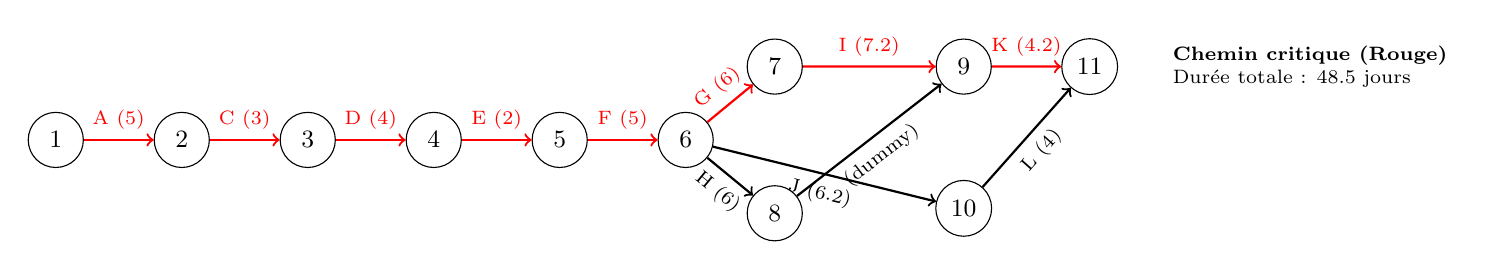
\begin{tikzpicture}[scale=0.85, state/.style={draw, circle, minimum size=0.7cm, fill=white, font=\small}, node distance=1.6cm]
    % Noeuds
    \node[state] (1) at (0,0) {1};
    \node[state] (2) [right of=1] {2};
    \node[state] (3) [right of=2] {3};
    \node[state] (4) [right of=3] {4};
    \node[state] (5) [right of=4] {5};
    \node[state] (6) [right of=5] {6};
    \node[state] (7) [above right of=6, yshift=-0.2cm] {7};
    \node[state] (8) [below right of=6, yshift=0.2cm] {8};
    \node[state] (9) [right of=7, xshift=0.8cm] {9};
    \node[state] (10) [below of=9, yshift=-0.2cm] {10};
    \node[state] (11) [right of=9] {11};
    
    % Flèches
    \draw[->, thick, red] (1) -- node[above] {\scriptsize A (5)} (2);
    \draw[->, thick, red] (2) -- node[above] {\scriptsize C (3)} (3);
    \draw[->, thick, red] (3) -- node[above] {\scriptsize D (4)} (4);
    \draw[->, thick, red] (4) -- node[above] {\scriptsize E (2)} (5);
    \draw[->, thick, red] (5) -- node[above] {\scriptsize F (5)} (6);
    
    \draw[->, thick, red] (6) -- node[above, sloped] {\scriptsize G (6)} (7);
    \draw[->, thick] (6) -- node[below, sloped] {\scriptsize H (6)} (8);
    \draw[->, thick] (6) -- node[below, sloped] {\scriptsize J (6.2)} (10);
    
    \draw[->, thick, red] (7) -- node[above] {\scriptsize I (7.2)} (9);
    \draw[->, thick] (8) -- node[below, sloped] {\scriptsize (dummy)} (9);
    
    \draw[->, thick, red] (9) -- node[above] {\scriptsize K (4.2)} (11);
    \draw[->, thick] (10) -- node[below, sloped] {\scriptsize L (4)} (11);
    
    % Dates au plus tôt et au plus tard (légende à côté)
    \node[draw=none, fill=none, right of=11, xshift=1.2cm, align=left, font=\scriptsize] {
        \textbf{Chemin critique (Rouge)} \\
        Durée totale : 48.5 jours
    };
\end{tikzpicture}
}
\caption{Réseau PERT et chemin critique}
\label{fig:pert_pfa}
\end{figure}

\section{Conclusion}
Ce premier chapitre a permis d'ancrer notre projet dans la réalité socio-économique marocaine. L'étude de l'existant a mis en lumière les besoins de sécurité et d'interactivité auxquels ManageraHub doit répondre. En planifiant rigoureusement le projet sous la méthodologie 2TUP et en validant notre chemin critique de 48,5 jours, nous disposons d'un cadre stable pour aborder la conception technique du système.
\newpage
